\section{mo\-Next\-Move$<$ M $>$ Class Template Reference}
\label{classmo_next_move}\index{moNextMove@{moNextMove}}
Class which allows to generate a new move ({\bf mo\-Move}{\rm (p.\,\pageref{classmo_move})}).  


{\tt \#include $<$mo\-Next\-Move.h$>$}

Inheritance diagram for mo\-Next\-Move$<$ M $>$::\begin{figure}[H]
\begin{center}
\leavevmode
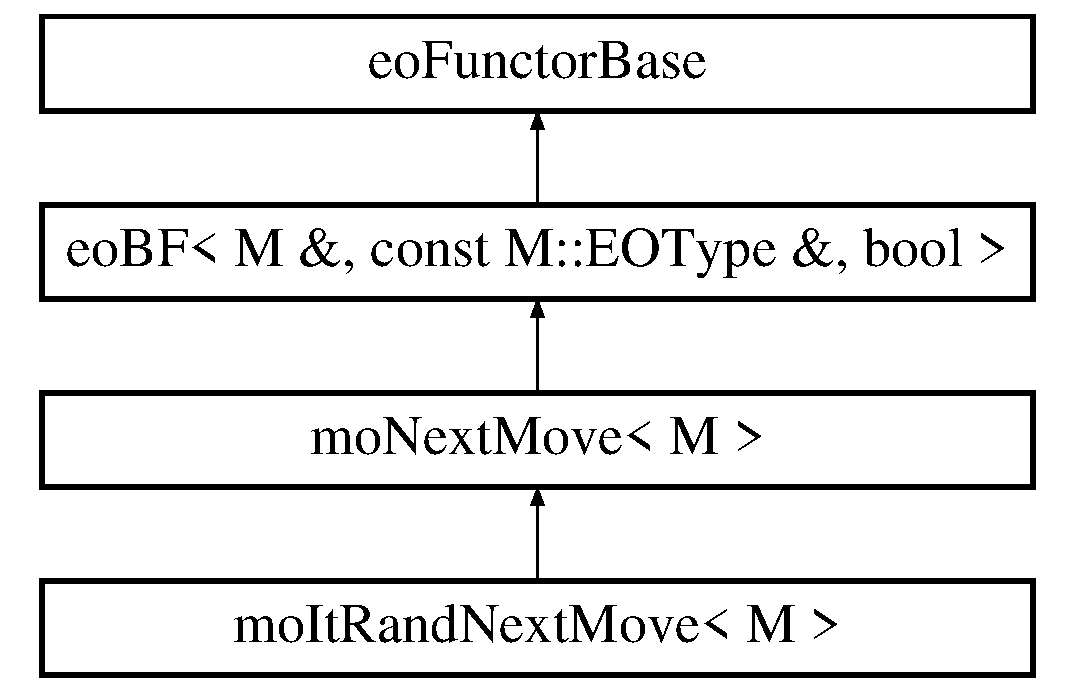
\includegraphics[height=4cm]{classmo_next_move}
\end{center}
\end{figure}


\subsection{Detailed Description}
\subsubsection*{template$<$class M$>$ class mo\-Next\-Move$<$ M $>$}

Class which allows to generate a new move ({\bf mo\-Move}{\rm (p.\,\pageref{classmo_move})}). 

Useful for the explorer (for {\bf mo\-TS}{\rm (p.\,\pageref{classmo_t_s})} or {\bf mo\-HC}{\rm (p.\,\pageref{classmo_h_c})}). Does nothing... An object that herits from this class needs to be designed for being used. 



Definition at line 47 of file mo\-Next\-Move.h.

The documentation for this class was generated from the following file:\begin{CompactItemize}
\item 
mo\-Next\-Move.h\end{CompactItemize}
